\documentclass[tikz, border=5mm]{standalone}
\usetikzlibrary{arrows.meta, positioning}
\begin{document}
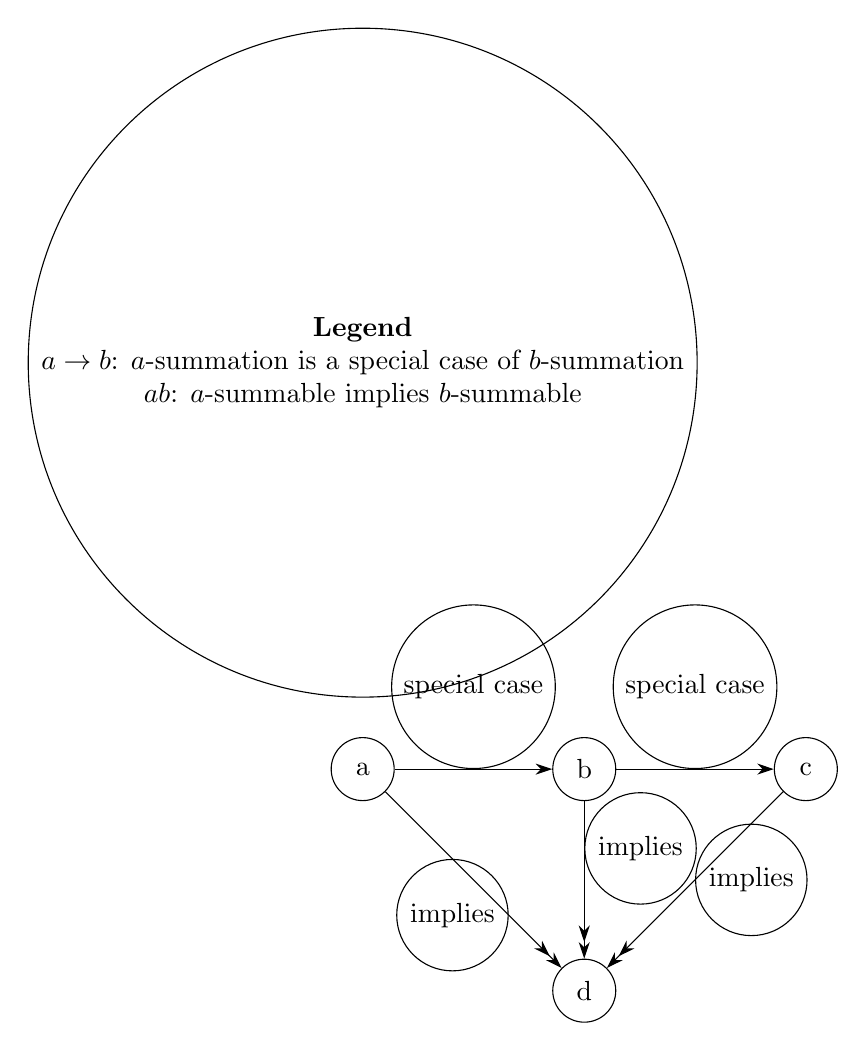
\begin{tikzpicture}[
    node distance=2cm,
    every node/.style={circle, draw, minimum size=0.8cm},
    >={Stealth[width=4pt,length=6pt]},
    single arrow/.style={->},
    double arrow/.style={->>},
    label distance=2pt
]
% Nodes
\node (a) {a};
\node (b) [right=of a] {b};
\node (c) [right=of b] {c};
\node (d) [below=of b] {d};
% Relationships
\draw[single arrow] (a) -- node[above] {special case} (b);
\draw[single arrow] (b) -- node[above] {special case} (c);
\draw[double arrow] (a) -- node[left, pos=0.7] {implies} (d);
\draw[double arrow] (b) -- node[right, pos=0.3] {implies} (d);
\draw[double arrow] (c) -- node[right] {implies} (d);
% Annotations
\node[above=0.5cm of a, anchor=south, align=center]
    {\textbf{Legend}\\$a \to b$: $a$-summation is a special case of $b$-summation\\
     $a \twoheadrightarrow b$: $a$-summable implies $b$-summable};
\end{tikzpicture}
\end{document}